\documentclass[letterpaper,times,numbered,print,custommargin]{Classes/PhDThesisPSnPDF}
% ******************************************************************************
% ******************************* Class Options ********************************
% *********************** See README for more details **************************
% ***   https://github.com/kks32/phd-thesis-template/blob/master/README.md   ***
% ******************************************************************************


% ********************************** Preamble **********************************
% Preamble: Contains packages and user-defined commands and settings
% ******************************************************************************
% ****************************** Custom Margin *********************************

% Add `custommargin' in the document class options to use this section
% Set {innerside margin / outerside margin / topmargin / bottom margin}  and
% other page dimensions
\ifsetMargin
\else
% \RequirePackage[left=37mm,right=30mm,top=35mm,bottom=30mm]{geometry}
    \RequirePackage[left=30mm,right=20mm,top=30mm,bottom=20mm]{geometry}
    \setFancyHdr % To apply fancy header after geometry package is loaded
\fi

% % *****************************************************************************
% % ******************* Fonts (like different typewriter fonts etc.)*************
% 
% % Add `customfont' in the document class option to use this section
% \ifsetFont
% \else
%     % Set your custom font here and use `customfont' in options. Leave empty to
%     % load computer modern font (default LaTeX font).  
%     \RequirePackage{libertine} 
% \fi

% *****************************************************************************
% *************************** Bibliography  and References ********************

%\usepackage{cleveref} %Referencing without need to explicitly state fig /table

% Add `custombib' in the document class option to use this section
\ifsetBib % True, Bibliography option is chosen in class options
\else % If custom bibliography style chosen then load bibstyle here
    \RequirePackage[square, sort, numbers, authoryear]{natbib} % CustomBib
\fi

% changes the default name `Bibliography` -> `References'
\renewcommand{\bibname}{References}
\renewcommand*{\bibfont}{\footnotesize}


% *****************************************************************************
% *************** Changing the Visual Style of Chapter Headings ***************
% Uncomment the section below. Requires titlesec package.

\RequirePackage{titlesec}

% http://tex.stackexchange.com/questions/30757/change-the-word-chapter-to-something-else
 \renewcommand{\chaptername}{}


% \titleformat{\chapter}{\filleft\normalfont\huge\bfseries}{\thechapter }{30pt}{\huge}
% \titlespacing*{\chapter}{0pt}{50pt}{20pt}

% \newcommand{\PreContentTitleFormat}{\titleformat{\chapter}[display]{\scshape\Large}
% {\Large\filleft{\chaptertitlename} \Huge\thechapter}
% 
%  {1ex}{}
%   [\vspace{1ex}\titlerule]}
%   \newcommand{\ContentTitleFormat}{\titleformat{\chapter}[display]{\scshape\huge}
%   {\Large\filleft{\chaptertitlename} \Huge\thechapter}{1ex}
%   {\titlerule\vspace{1ex}\filright}
%   [\vspace{1ex}\titlerule]}
%  \newcommand{\PostContentTitleFormat}{\PreContentTitleFormat}
%  \PreContentTitleFormat


% *****************************************************************************
% **************************** Custom Packages ********************************
% *****************************************************************************


% ************************* Algorithms and Pseudocode **************************

%\usepackage{algpseudocode} 


% ********************Captions and Hyperreferencing / URL **********************

% Captions: This makes captions of figures use a boldfaced small font. 
%\RequirePackage[small,bf]{caption}

\RequirePackage[labelsep=space,tableposition=top]{caption} 
\renewcommand{\figurename}{Fig.} %to support older versions of captions.sty

% ************************ Formatting / Footnote *******************************

%\usepackage[perpage]{footmisc} %Range of footnote options 


% ****************************** Line Numbers **********************************

%\RequirePackage{lineno}
%\linenumbers

% ************************** Graphics and figures *****************************

%\usepackage{rotating}
%\usepackage{wrapfig}
%\usepackage{float}
\usepackage{subfig} %note: subfig must be included after the `caption` package. 


% ********************************* Table **************************************

%\usepackage{longtable}
%\usepackage{multicol}
%\usepackage{multirow}
%\usepackage{tabularx}

\usepackage[table]{xcolor}
\usepackage{booktabs}
% \rowcolor{blue!10}

\usepackage{array}
% \begin{tabular}{| c | c |  >{\centering}m{5cm} |}



% ***************************** Math and SI Units ******************************

\usepackage{amsfonts}
\usepackage{amsmath}
\usepackage{amssymb}
%\usepackage{siunitx} % use this package module for SI units


% ******************************************************************************
% ************************* User Defined Commands ******************************
% ******************************************************************************


% ********************** TOC depth and numbering depth *************************

\setcounter{secnumdepth}{2}
\setcounter{tocdepth}{2}

% ******************************* Nomenclature *********************************

% To change the name of the Nomenclature section, uncomment the following line

%\renewcommand\nomname{Symbols}


% ********************************* Appendix ***********************************

% The default value of both \appendixtocname and \appendixpagename is `Appendices'. 
% These names can all be changed via: 

%\renewcommand{\appendixtocname}{List of appendices}

%\renewcommand{\appendixname}{Appndx}




% ******************************************************************************
% ********************************* Ghant Chart 
\usepackage{tikz}
\usepackage{Classes/gantt}
 \usepackage{pdflscape}


% ******************************************************************************
% ********************************      
% http://stackoverflow.com/questions/491904/
% latex-how-to-remove-blank-pages-coming-between-two-chapters-in-appendixname
\let\cleardoublepage\clearpage

% *****************************************************************************
% ********************************  COMPACT ITEMIZE   
% http://stackoverflow.com/questions/4968557/latex-very-compact-itemize
% \usepackage{enumitem}
% ...
% \begin{itemize}[noitemsep,topsep=0pt,parsep=0pt,partopsep=0pt]
%  \item 
% \end{itemize}
\usepackage{enumitem}



% *****************************************************************************
% ********************************  FONT SIZE OF THE TITLE   
\usepackage{anyfontsize}

% *****************************************************************************
% ************************  TWO COLUMS FOR SUPERVISORS SIGNS    
\usepackage{multicol}
% \begin{multicols}{2}
% Column 1
% \columnbreak
% Column 2
% \end{multicols}
\usepackage{blindtext}


% *****************************************************************************
% *************************** Typing shortcuts 
  
\newcommand{\ANN}[0]{\textsf{ANN}}
\newcommand{\librER}[0]{\textsf{LibrE Robotics}}

\newcommand{\ANNversion}[0]{1.1}
\newcommand{\librERversion}[0]{0.1}

\newcommand{\ANNyear}[0]{2010}
\newcommand{\librERyear}[0]{2014}


% *****************************************************************************
% ***************************  \textcopyleft 
\usepackage{textcomp}



\graphicspath{{Figs/}{Figs/}}


% ******************************************************************************
% ************************ Thesis Information & Meta-data **********************
%% The title of the thesis
% 
\title{
LibrE Robotics: \\
\vspace{5mm}
\Large{Educational Robotics for\\
	Learning and Sharing Knowledge \\
	to Build Conditions for a Better World}\\
}

%% The full name of the author
% \author{generally speaking a mammal who}
% \author{WANT TO CHANGE THE WORLD FOR BETTER LIVING CONDITIONS}

 \crest{
\includegraphics[scale=1.3]{Preamble/LibrERobotics_logo.png}}


%% You can redefine the submission text:
% Default as per the University guidelines: This dissertation is submitted for
% the degree of Doctor of Philosophy
\renewcommand{\submissiontext}{
% PhD Research Proposal
}

%% Submission date
\degreedate{
14th of June 2014 \\ 
Document Release 001 \\ 
\url{https://sites.google.com/site/librerobotics/}
} 

%% Meta information
\subject{LaTeX} 
\keywords{{LaTeX} } 


% ***************************** Abstract Separate ****************************** 
% To printout only the titlepage and the abstract with the PhD title and the 
% author name for submission to the Student Registry, use the abstract option in
% the document class. 
\ifdefineAbstract
 \includeonly{Abstract/abstract} 
\else
\fi


% ******************************** Front Matter ********************************
\begin{document}
\frontmatter
\begin{titlepage}
\maketitle
\end{titlepage}
%*****************************************************************************************
%*********************************** Abstract ********************************************
%*****************************************************************************************

\begin{abstract}
The aim of this document is to point out the importance of the development of a free 
world-class education in Robotics for kids by proposing, designing and building low-cost 
robots with high standards of quality. On account of Open Source Software and Hardware 
is freely licensed to use, copy, study and change in any way, ten open-source educational 
robots were reviewed. Consequently, it has been proposed a low-cost robot that is based on 
an Arduino UNO board, two hacked continuous servos, and some extra material such as 
recycled CDs, glue gun, etc.; the total cost of the material in local stores is around 
\$  699 Mexican Pesos ($\approx$ \$ 53.86 USD). It has also been 
proposed that Ardublock is going to be the main programming language for the low-cost 
robot considering that it is a programming tool which is very interactive and simple to 
use for inexperienced users. Independently, however, of the low cost of the proposed 
robot, it is robust for basic activities, namely: left and right rotations, movements in 
forward and backward directions to name but a few, and more importantly it is also being 
capable of recognising voice control commands. On the other hand, since {\librER} has 
been thought to be a non-profit organization, people from different fields of study can 
help us to improve the project in different ways by which possible activities and 
open-source software to use have been proposed. As a timeline, a ghantt chart is also 
presented in which six tasks have been considered to be implemented in 16 months: namely;
T1) development of the low-cost robot; T2) implementation of new tools in Ardublock;
T3) development of the speech recognition tool; 
T4) integration of the tasks T1, T2 and T3;
T5) design of the first workshop, and 
T6) evaluation of the complete project.
Finally, as a future work two projects have been briefly reviewed: 1) the implementation 
of inductive wireless power systems to get rid of batteries that are enviromental 
unfriendly and the USB cable that is an issue for the mobility of the robot, and 2) 
the importance of the facilities' enviroment that have a significant role in influencing 
participants for their academic performance and mainly that they can discover and develop 
their own capabitilies.
\end{abstract}


% *********************** Adding TOC and List of Figures ***********************
\tableofcontents

% \printnomenclature[space] space can be set as 2.5cm between symbol and
% description
% \printnomencl

% ******************************** Main Matter *********************************
\mainmatter

%*****************************************************************************************
%*********************************** First Chapter ***************************************
%*****************************************************************************************

\chapter{Introduction}  %Title of the First Chapter

% **************************** Define Graphics Path **************************
\graphicspath{{Chapter1/Figs/}{Chapter1/Figs/}}

\vspace{1mm}
\footnotesize {
\begin{flushright}
\textit{
Let us try teaching children \textbf{how to think} instead of what to think.
}\\
\end{flushright}
}
\vspace{1mm}


%-----------------------------------------------------------------------------------
\section{What is {\librER}?}
%-----------------------------------------------------------------------------------
{\librER} is inspired by KHAN academy \cite{KHAN} which is a non-profit organization
with the goal of changing education for the better. In the same fashion, {\librER} 
has also been thought to be a non-profit organization in which the main goals are 
fivefold:
\begin{itemize}[noitemsep,topsep=0pt,parsep=0pt,partopsep=0pt]
 \item to contribute to the development of a free world-class education in Robotics 
 for anyone anywhere;
 \item to design and build low-cost robots with high standards of quality;
 \item to improve current open source software projects so as to be more approachable 
 by inexperienced users; 
 \item to design free access material in educational Robotics, and develop activities 
 where organization and cooperation of the participants can foster
 possible solutions for environmental, social and healthcare issues; and
 \item to design and build environments where participants can discover and
 develop their own capabilities.
\end{itemize}

{\librER} will provide software and hardware for educational robots that are extremely 
reliable (robust), modifiable, and very cheap in order to be accessible to anyone and 
to enable a much more rapid development of the community.

In addition to that, {\librER} has been adopted the philosophy of free software 
foundation, since free and open-source software and hardware licences state that anyone 
is freely licensed to use, copy, study and change in any way, and the source code is 
openly shared so that users are encouraged to voluntarily improve the design of the 
software. As Meyer \cite{Meyer2003} put it,``Libre software offers scientists the 
possibility of sharing with their peers how they have solved problems. This, of course 
is basic for the evolution of science; but libre software goes beyond tha and makes 
this happen in a cost-effective way.'' 

%-----------------------------------------------------------------------------------
\section{What are the Benefits for Learning and Sharing with {\librER}?}
%-----------------------------------------------------------------------------------
There are many benefits that can be derived from {\librER}, mainly because the 
creation of strong links between industry, government, education and sociecity. 
Robotics is a multidisiplinary field in which mathematics, physicis, mechanics, 
computational science and electronics to mention but a few are applied.
Robotics applications have been proven to be many and these are ranging from 
agriculture to factory automation, from healthcare to education \cite{ashesirobotics2013}. 
Aditionally, robotics is a fascinating and fun way to develop creativity as well as the 
design, implementation, and integration of ideas that are essential for the development 
of skills that provides participants to cooperate and build conditions for a better world. 
Henceforth, similar projects of educational robotics that epitomise benefits for their 
communities are reviewed in the following section.

Valeria Larrar, a primary professor from Argentine, designed various workshops in educational 
robotics for participants between 10 and 15 years old in public schools. Valeria at a TED 
talk \cite{Larrart2013} in October 2013 mentioned that having seen the succefulness and 
possibilities of his first workshop, the educational ministery of Argentine afforded her 
school to buy 30 Robotics LEGO kits. It is important to mention that one of the goals 
for workshops is to tackle common issues in the community, for example, having known 
the problem of usefulness of traffic lights in busy highways, students built an 
automatized bridge to transport mainly disable people. Valeria emphasised that the power 
of interest is really great that what it looks like a professor guiding his pupils 
(Figure \ref{fig:educationalroboticsprojects}), in reality that person is the school 
caretaker who is delighted by the educational robotics software.
\begin{figure}[htbp!] 
\centering    
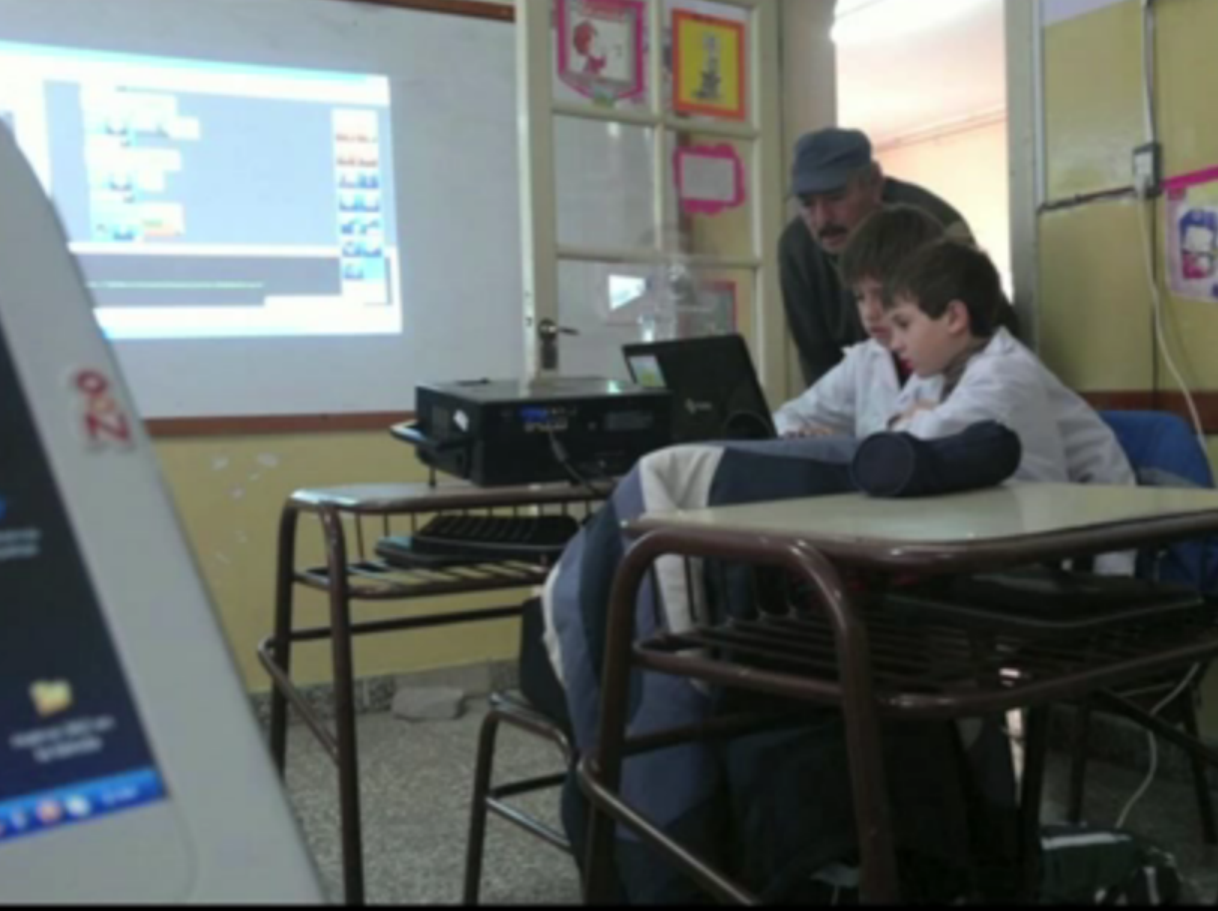
\includegraphics[width=0.4\textwidth]{chicos_and_conserge.png}
\caption[PA]{A school caretaker watching the boys using educational robotics software.}
\label{fig:educationalroboticsprojects}
\end{figure}
Valeria's projects showed that by learning robotics, students can create many 
oportunities, relationships among parents and sibilings, friends, and most importantly
finding joyness and optimismn in doing something that they love.

Similarly, the Ashesi Robotics Experience (ARX), an annual robotics workshop in Africa,
is designed to provide a stimulating, fun and refreshing environment 
for students to learn robotics \cite{ARX2013}. At ARX 2013 mentors were selected
from Ashesi University College who possessed the right set of skills and attributes 
to mentor, train, and take responsability of students. During one week, students 
were working on building Lollybots and LEGO Mindstorm Robots and 
on the last day, the community where invited to see students' projects 
so as to show that Robotics can be used as a way of critical thinking to solve social 
problems.
ARX also provides statistics of the participants in which the number of boys were 34, 
representing 57\% of participants, while girls were 26, representing the other 43\%. 
Participants were between the ages of 15 to 21 and came from all nine regions of Ghana, 
as well as two international students from Ethiopia and Swaziland 
(Figure \ref{fig:arx2013}).
\begin{figure}[htbp!] 
\centering    
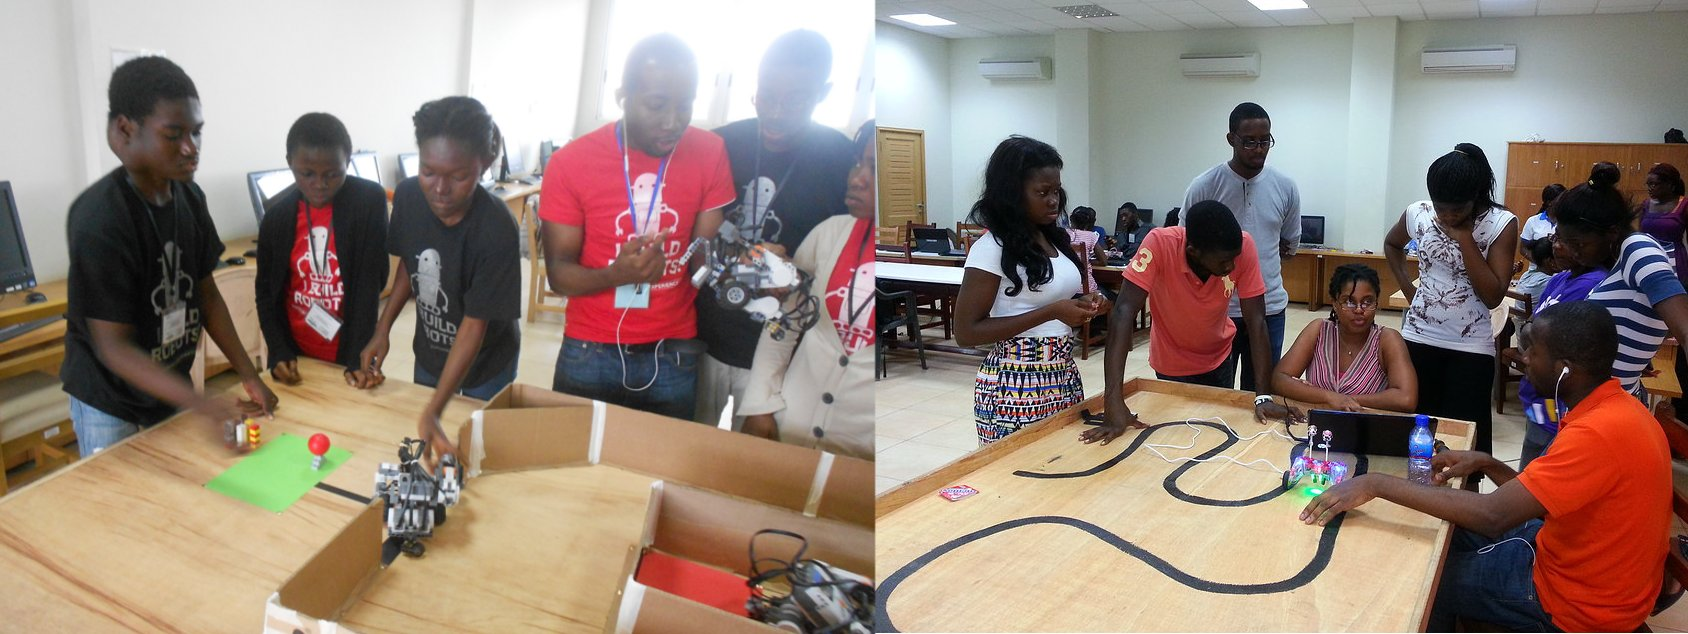
\includegraphics[width=0.75\textwidth]{arx2013_main.jpg}
\caption[PA]{Ashesi Robotics Experience Workshop 2013}
\label{fig:arx2013}
\end{figure}
Additionally, Ashesi Robotics posted several final projects at their webpage 
\cite{ashesirobotics2013}, for instance, exploration robots,
Planning in Dynamic Environment, Building a Sorter Robot, Follow the leader,
Tic-tac-toe, Dynamic balancing and Robot Navigation using colors as road signs.
It is important to note that all projects were documented by using 
these outline: Introduction, Approach, Algorithm, Results, Conclusion, and Appendix.

Having checked the positive benefits, one can see that many of the previos-mentioned 
projects were implemented with LEGO Mindstorm Robots which represent a signigicantly 
economical inversion. To this end, The African Robotics Network (AFRON) 
community presented a project called ``Ultra Affordable Educational Robot'' in 
which many participants around the world are called to present their robot designs 
that can inspire young children worldwide about Science, Technology, Engineering, 
and Math \cite{AFRON2014}. One of the primary goals for Ultra Affordable Educational 
Robot is to make robots that are more functional, more realiable, easier to use, less 
expensive and easier to manufacture. At the AFRON Design Challenge 3 categories were
considered: 
1) hardware 2) software, or 3) curriculum (Figure \ref{fig:afron2014}). First places 
are going to be cited, however, second and third places are worth of reviewing in the 
future. Both in the hardware and curriculum categories, The MIT SEG: An Origami-Inspired 
Segway Robot won the first place mainly because of  its accesible price of 
approximately \$20 US dollars 
\cite{MITPrintableRobot2013}. MIT SEG's software is based on ardublock
\cite{Ardublock2013}  for which activities were taught using finite state machine 
concepts. In the software category, AERobot: an Affordable Education Robot won the first 
place \cite{AERobot2013}. AERobot's software is based on Minibloqs, a graphical 
programming environment \cite{minibloq2011}, that allow novice programmers to easily 
program their little Robot.
\begin{figure}[htbp!] 
\centering    
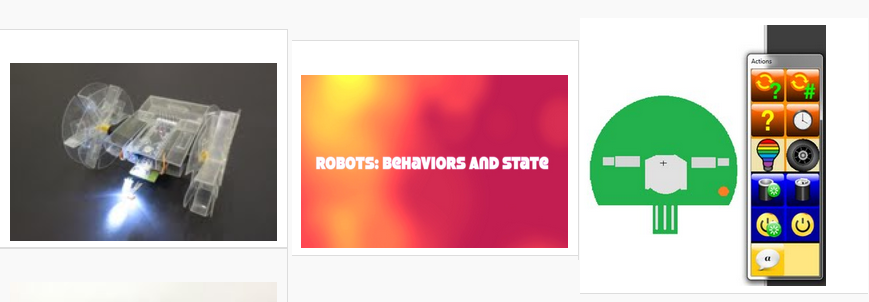
\includegraphics[width=0.8\textwidth]{afron2014}
\caption[PA]{First places at the AFRON Design Challenge: The MIT SEG, Behaviors and 
states with finite state machine concepts, and  AERobot's software based on minibloq
(from left to right).}
\label{fig:afron2014}
\end{figure}

It is also important to note that there are many related projects for educational robots, 
that are not open source software and hardware projects with high prices that are out 
of the current economical posibilities, for instance, Finch Robot \cite{finchrobot2014} 
and Bee-Bot \cite{bee-bot2014}; however, both provide a good references for lessons 
and software tools.
 % Introduction
%*****************************************************************************************
%*********************************** Second Chapter **************************************
%*****************************************************************************************
\chapter{Low-Cost Robot: Hardware and Software Requirements}
% **************************** Define Graphics Path **************************
\graphicspath{{Chapter2/Figs/}{Chapter2/Figs/}}

    
\vspace{10mm}
\footnotesize {
\begin{flushright}
\textit{
La semplicit\'a \'e l\'ultima sofisticazione.
}\\
Leonardo Da Vinci
\end{flushright}
}
\vspace{10mm}

%----------------------------------------------------------------------
\section{Hardware Requirements}
%----------------------------------------------------------------------
Different educational robots are reviewed in order propose a low-cost robot for {\librER}.
\subsection{A Review of Educational Robots}
According to the Finch Robot which was proposed by a lab at Carnegie Mellon University
\cite{finchrobot2014}, there are five features that are essential
to be considered when one is designing educational robots:
\begin{itemize}[noitemsep,topsep=0pt,parsep=0pt,partopsep=0pt]
 \item Works everywhere;
 \item Rich Interactivity (Programming should be less tedious);
 \item Aesthetically Appealing;
 \item Robust Hardware; and,
 \item Minimal Curricular Changes.
 \end{itemize}
 The Finch Robot hardware includes: light, temperature, and obstacle sensors,
 Accelerometers, Motors, Buzzer, Full-color beak LED, 
 Pen mount for drawing capability and Plugs into USB port (Figure \ref{fig:finch}).
 One of the main advatange of the Finch robot is that use the USB port as a power
device thus there are no batteries to charge and robot behavior can not be affected
by on-board power levels. The Finch Robot cost is \$ 99.00 USD and it has got both 
hardware and software as closed licences.
\begin{figure}[htbp!] 
\centering    
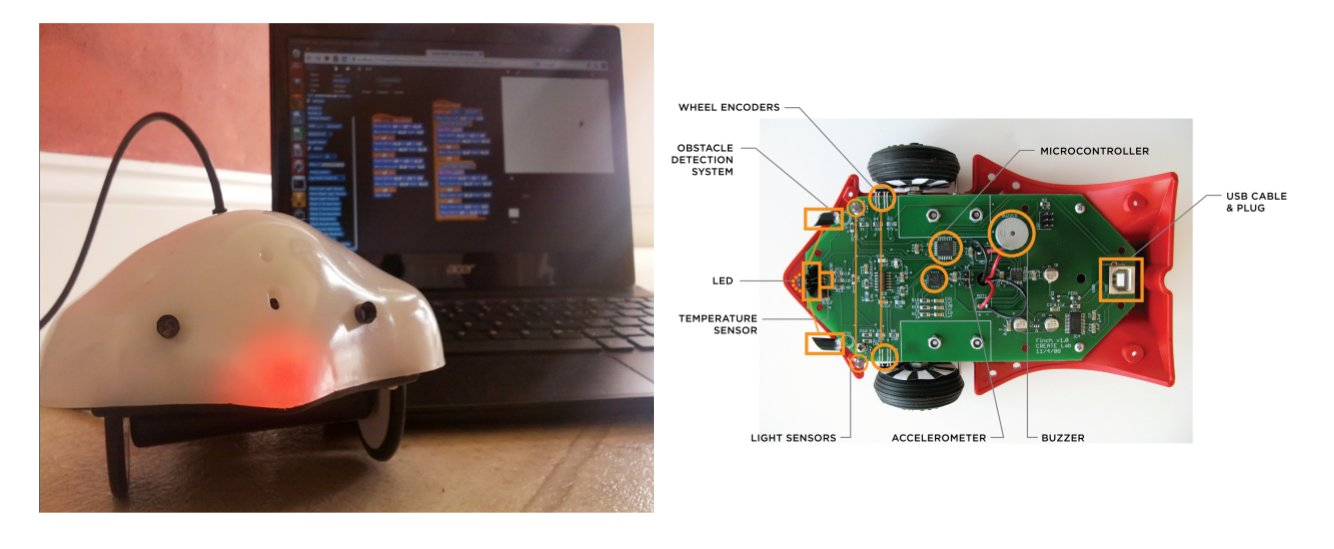
\includegraphics[width=0.9\textwidth]{finch_ps}
\caption[PA]{Finch Robot (left) and Finch' Sensors (right)}
\label{fig:finch}
\end{figure}

Bee-Bot  is a robot designed for use by young children \cite{bee-bot2014}. 
Directional keys are used to enter up to 40 commands which send Bee-Bot forward, back, 
left, and right (Figure \ref{fig:beebot}). Pressing the green GO button starts Bee-Bot 
on its way. Bee-Bot blinks and beeps at the conclusion of each command to allow children 
to follow Bee-Bot through the program they have entered and then confirms its completion 
with lights and sound. Bee-Bot is powered by a built-in rechargeable battery. Recharging 
is done via a standard USB recharger or USB computer port. Bee-Bot cost is \$89.95.
Additionally, a full line of Bee-Bot materials are available to enhance teaching and 
learning with Bee-Bot in the classroom: Bee-Bot lessons \$100.00, problem-solving with 
Bee-Bot \$100.00, and mats from \$29.95 to \$79.95. 
\begin{figure}[htbp!] 
\centering    
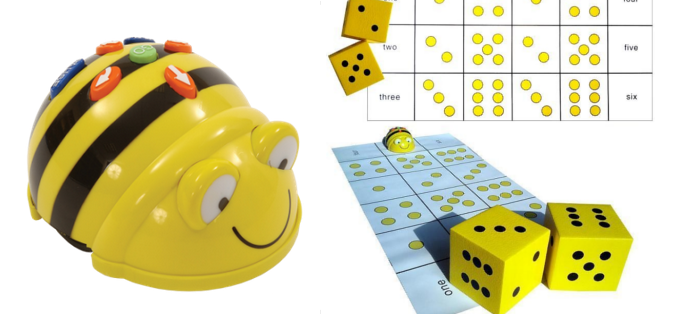
\includegraphics[width=0.5\textwidth]{beebotr}
\caption[PA]{Beebot: Robot (left) and Dice Mat (right).}
\label{fig:beebot}
\end{figure}
 
On the other hand, Thymio II robot is an open hardware and open source project 
\cite{timio}. Thymio II has got over 20 sensors, 40 lights, 2 motors 
(Figure \ref{fig:th}). It occupies a Micro-USB cable for charging and programming.
Thymio II Robot can be used with the integrated behaviours: Friendly (green), Explorer 
(yellow), Fearful (red), Investigator (cyan), Obedient (purple), and Attentive (blue).	
Thymio II Robot can also behave as : Slope avoidance, Balancing on a ball, Musical 
instrument, Light show, Positions in English, Thymio top model, Thymio as a dragon, 
Drawing machine, Learning commands, Special Effects and Light painting. Nonetheless, 
Thymio II's price is \$189 USD which is higher than Finch' Robot cost of \$ 99.00 USD.
\begin{figure}[htbp!] 
\centering    
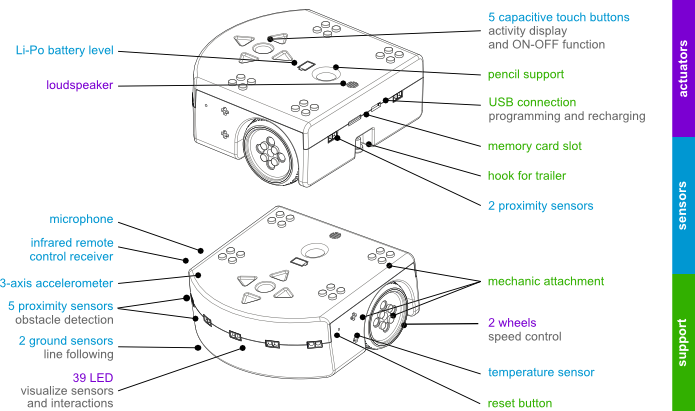
\includegraphics[width=0.6\textwidth]{thymioII-sensor-actuator-color-en}
\caption[PA]{Thymio II Sensor Actuators}
\label{fig:th}
\end{figure}
   

 
Androutsopoulos \emph{et at.}  \cite{Androutsopoulos2014} at the Department of Computer 
Science at Middlesex University from London have designed the MIddlesex Robotic plaTfOrm 
(MIRTO) (Figure. \ref{fig:RacketRobot}) which is an open-source platform built using 
Raspberry Pi, Arduino, and Racket as the core coordination mechanism. Robot's 
hardware has got two platforms: 1) base platform: two HUB-ee wheels with motors and 
encoders (to measure actual rotation), front and rear castors, two bump sensors, an array 
of six infra-red sensors, a rechargeable battery pack, an Arduino microcontroller board;
2) top layer: a Raspberry Pi connected to the Arduino, Linux with Racket (current version 
5.93), USB-WiFi adapter for SSH and network. Additional: cameras, microphones and text to 
speech with speakers. Since it is an educational project, it is not available for being 
bought; however, robot's hardware and software provide a good refeerence.
 \begin{figure}[htbp!] 
\centering    
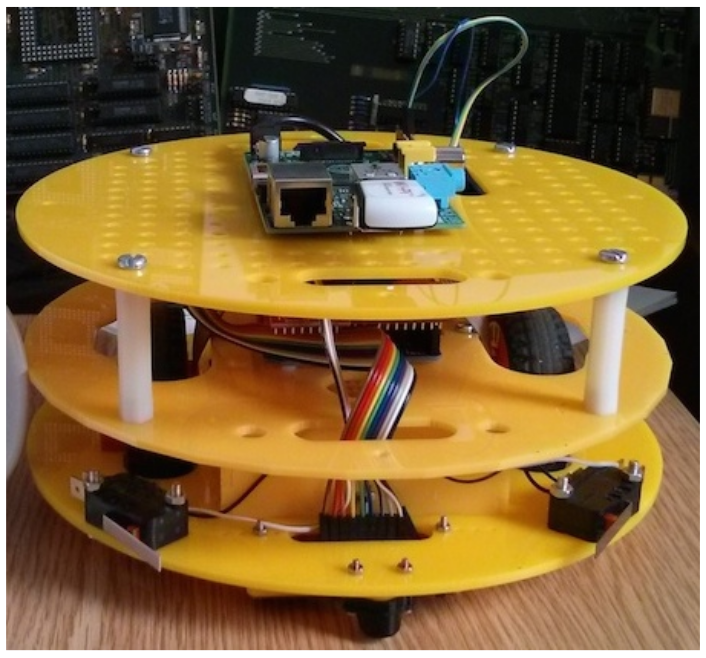
\includegraphics[width=0.4\textwidth]{TheMiddlesexRoboticPlatform}
\caption[PA]{MIddlesex Robotic plaTfOrm (MIRTO)}
\label{fig:RacketRobot}
\end{figure}
 
Equally important, Lil'Bot, a low-cost, open-source, Arduino-compatible balancing robot 
for learning, hacking and delight \cite{lilbot}, is worth to cite since many of its 
features are quite similar to the aim of LibrE Robotics. The main robot characteristics 
are: 1) Arduino Uno compatible; 2) Front, right and left obstable detection using IR 
LEDs; 3) Edge detection using an IR LED; 4) A buzzer plays musical tones and astromech 
droid sounds; 5) Wheel encoders for precise odometry-based control; and 6) the most 
important feature is that Lil' Bot project is released as Open-source hardware and 
software (Left Figure \ref{fig:lilbot}).  More features are shown in Left Figure 
\ref{fig:lilbot}. Lil' Bot can alternatively be energised with an energy source that
is based on Hydrogen Fuel Cells designed by Open Fuel Cell. Lil' Bot is integrated with 
a matrix of LEDs so as to express emotions such as afraid, amused, angry, blissful, 
cool, crying, disappointed, embarrased happy, impatient, naughty, neutral, nonplussed,
outtraged, proud, resigned, sad, sarcastics, shocket, smiling and very sad 
(Right Figure \ref{fig:lilbot}). Since it is a project under development, there is no 
price.
\begin{figure}[htbp!] 
\centering    
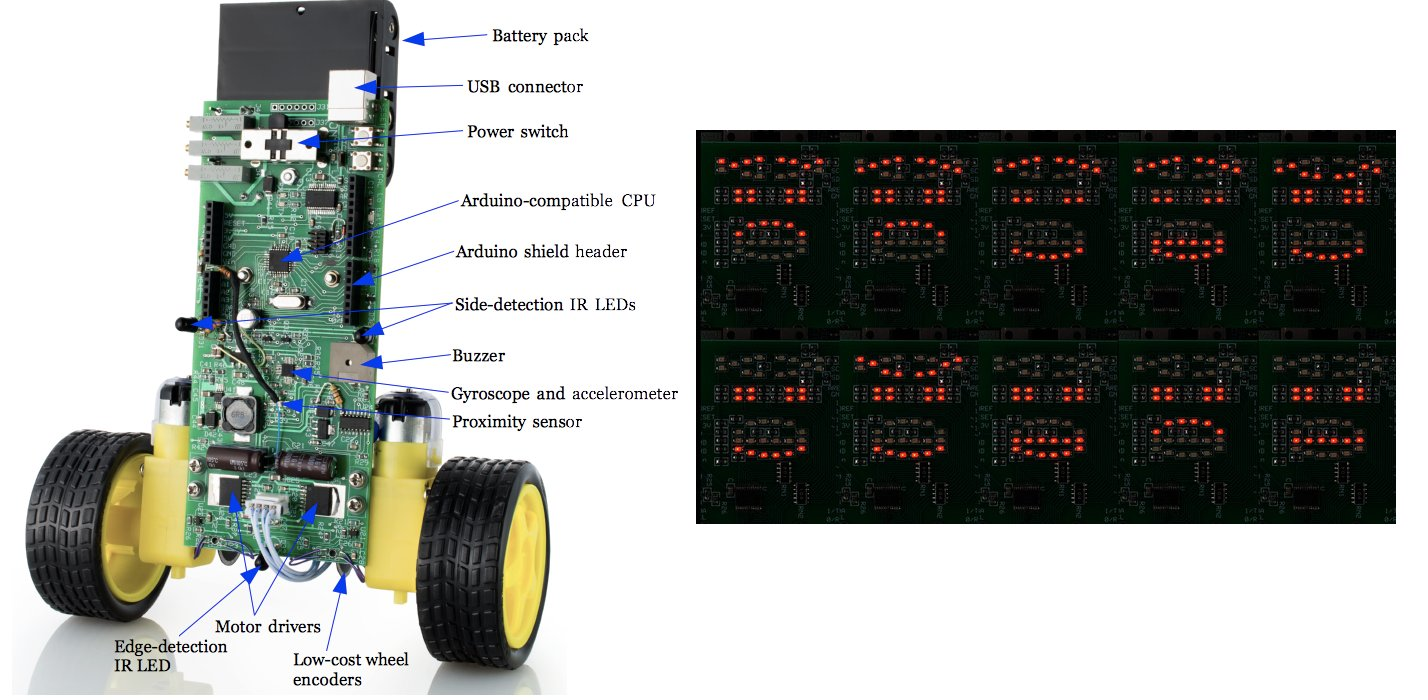
\includegraphics[width=0.8\textwidth]{lilbot}
\caption[PA]{Lil' Bot: Prototype (left), Emotion-like LED display (right)}
\label{fig:lilbot}
\end{figure}

Sparki is an affordable, easy to use, and fun intro to programming, electronics, and 
robotics \cite{sparki}. Sparki is affordable, featured-packed, open-source Arduino robot. 
Sparki comes with a bluetooth module, and array of onboard sensors, precise geared 
stepper motors, a motorized gripper to mention but a few (Figure \ref{fig:sparki}).
Sparki has got the following features: 
1) Ultrasonic distance sensor (get distance from Sparki to walls/objects);
2) 3-Axis Accelerometer (pick-up detection, fall detection, hill climbing);
3) 3-Axis Magnetometer (sense the magnetic field around Sparki, coordinate with 
accelerometer to detect compass heading);
4) Light-sensing phototransistors (light following, darkness seeking);
5) Line-following and edge detection sensors (mazes, line follow, sumo);
6) 128X64 Graphic LCD;
7) RGB LED (RGB = generate any color);
8) Buzzer (beeping, booping, and musical tones);
9) IR Transmitter (like your TV remote control);
10) IR Receiver (like your TV);
11) IR Remote control (lots of buttons to control Sparki with);
12) TTL Serial port for expansion (talk to an Arduino/Raspberry Pi);
13) Bluetooth Serial Module;
14) Powered by 4xAA batteries (not included); and,
15) Geared stepper motors (precise, measured movement down to millimeters/ sub-degrees).
Furthermore, Arcrobotics have develop a module to learn about robotics and to test 
programming capabilities which are available at \cite{sparkisoftware}. Total cost of the 
robot is \$150 USD. Sparki is released as a open-source project; yet, there are no 
further information regarding the Chassis and PDB designs other than basic examples 
of its library.
\begin{figure}[htbp!] 
\centering    
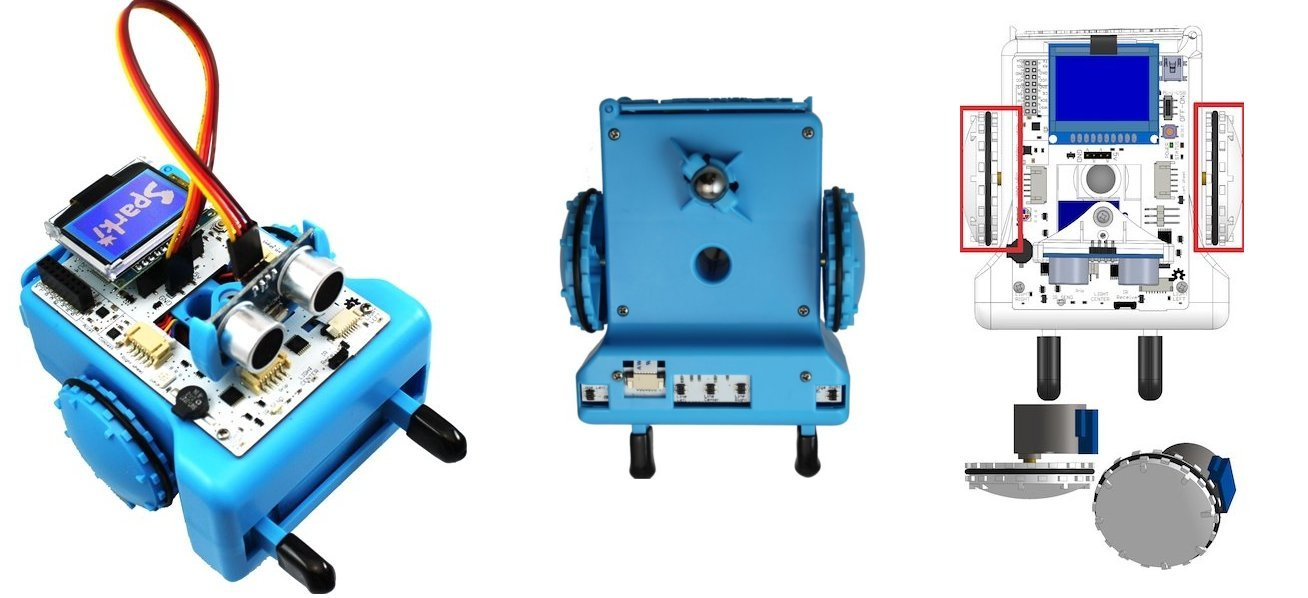
\includegraphics[width=0.7\textwidth]{sparki}
\caption[PA]{Sparki: Prototype (left), bottom part (center) and geared stepper motors 
(right)}
\label{fig:sparki}
\end{figure}
 
 
Mirobot is \textbf{a 100\% open source robot }to which PCB designs and schematics, 
firmware code, and chassis designs are available at \cite{mirobot}. Mirobot uses WiFi 
so that it is easy to get up and running and has been carefully designed to eliminate 
a lot of the difficulties that children  would normally have in building something like 
this (Figure \ref{fig:mirobot}). 
\begin{figure}[htbp!] 
\centering    
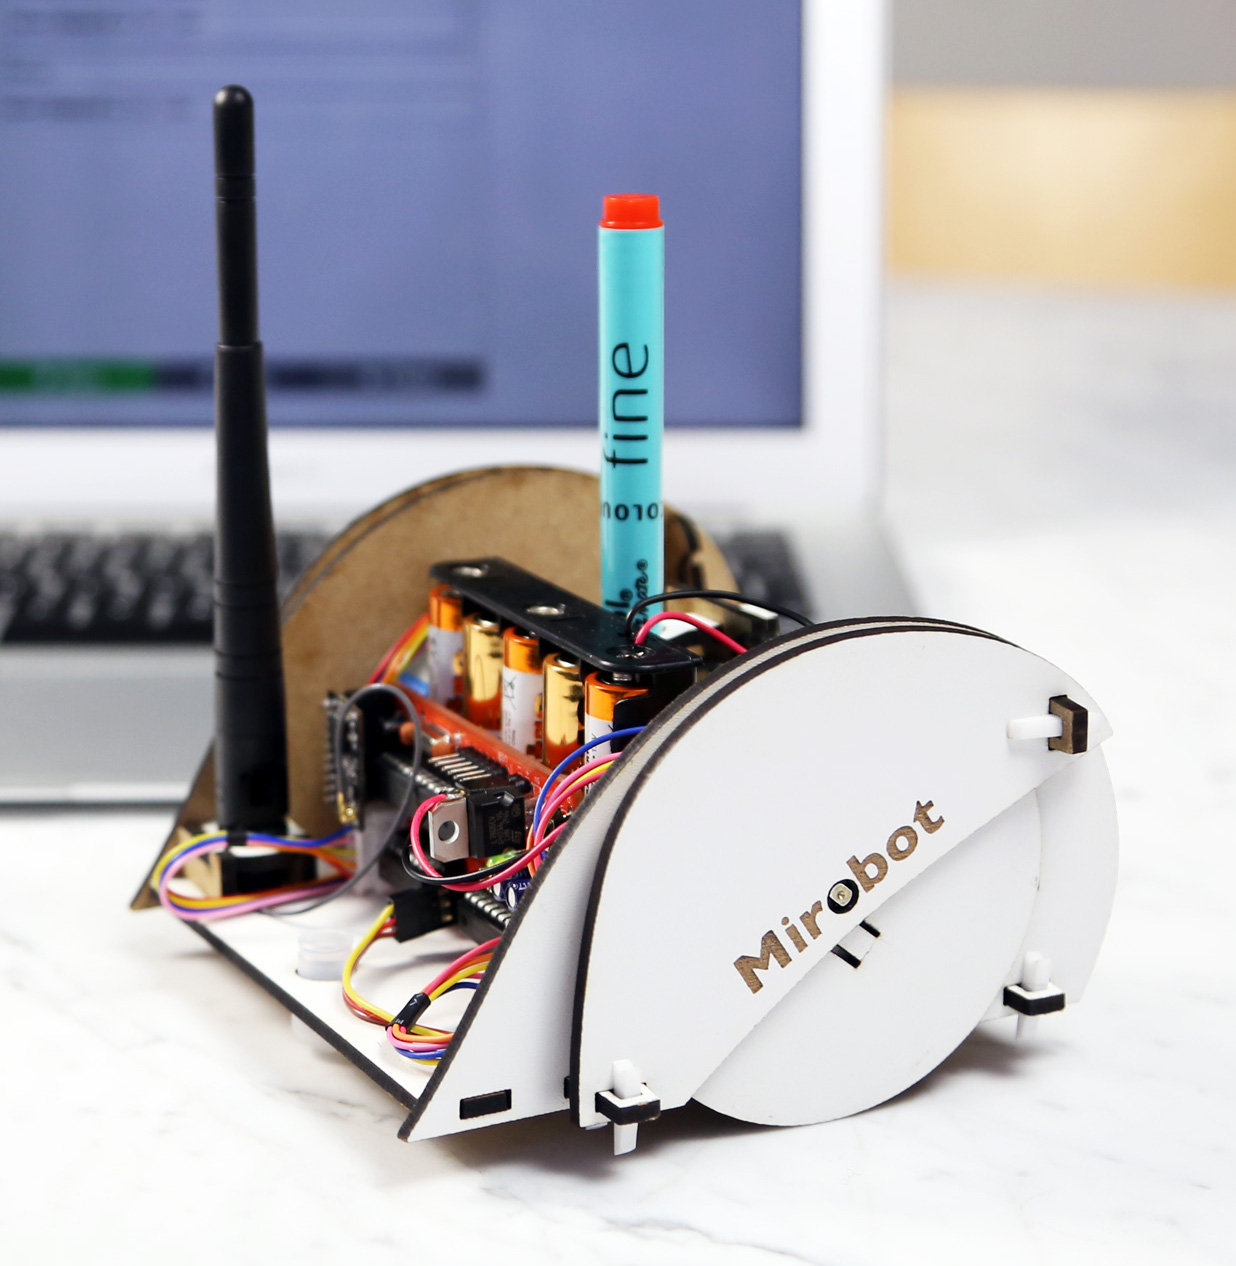
\includegraphics[width=0.5\textwidth]{mirobot}
\caption[PA]{Mirobot}
\label{fig:mirobot}
\end{figure}
 
 
In contrast to the previos-mentioned educational robots, low-cost robots are more 
suitable for the aim of the proyect. For instance, Bug-bot is build with five touch 
sensors, two antennea and three bumbers on 
the back (Figure \ref{fig:bugbot}). It has also got a Xbees wireless board to operate 
the robot with a joystick. Besides, DXF files are available to download in order to be 
easily sent to a laser cutter. PCB diagrams, arduino and processing code is also 
available \cite{bugbot}. 
\begin{figure}[htbp!] 
\centering    
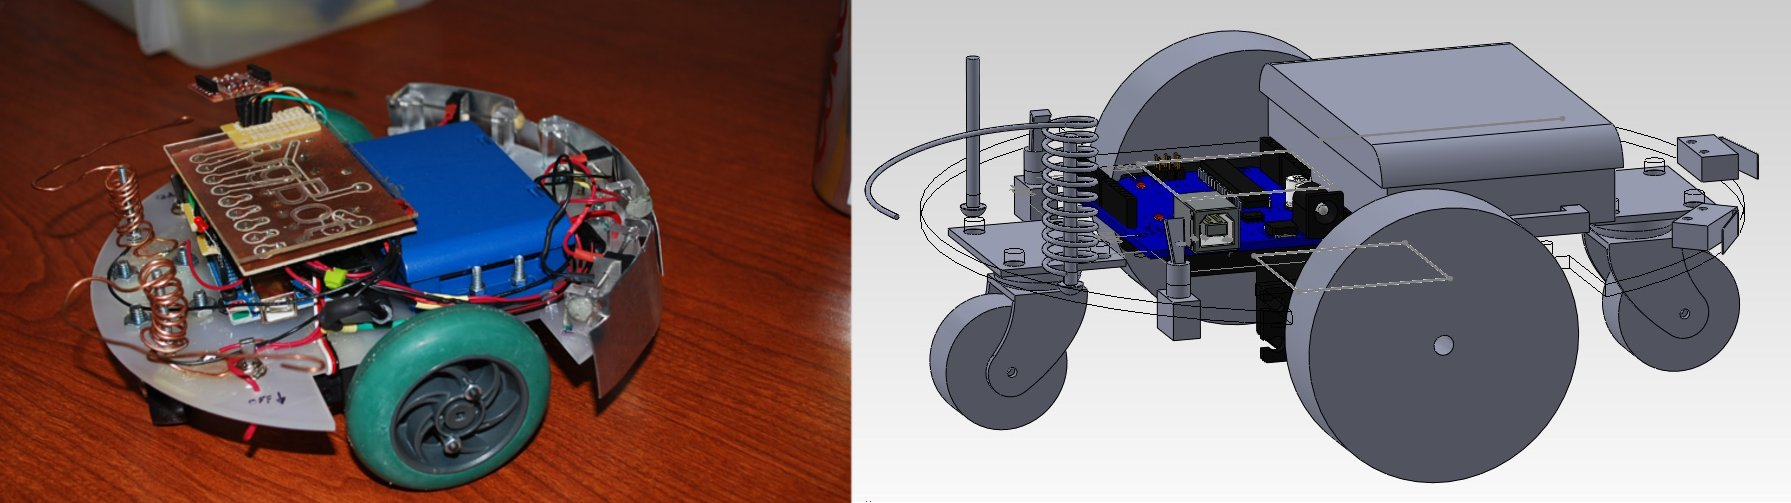
\includegraphics[width=0.75\textwidth]{bugbot}
\caption[PA]{Bug Bot: Prototype (left) CAD layout (right).}
\label{fig:bugbot}
\end{figure}

Boe Bot \cite{boebot}, an arduino line following robot, uses LEDs, light dependent 
resistors (LDRs), an arduino, and a boe bot chassis with 2 continuous rotation servos 
(Figure \ref{fig:boebot}). Nevertheless, the price is not presented in both prototypes.
\begin{figure}[htbp!] 
\centering    
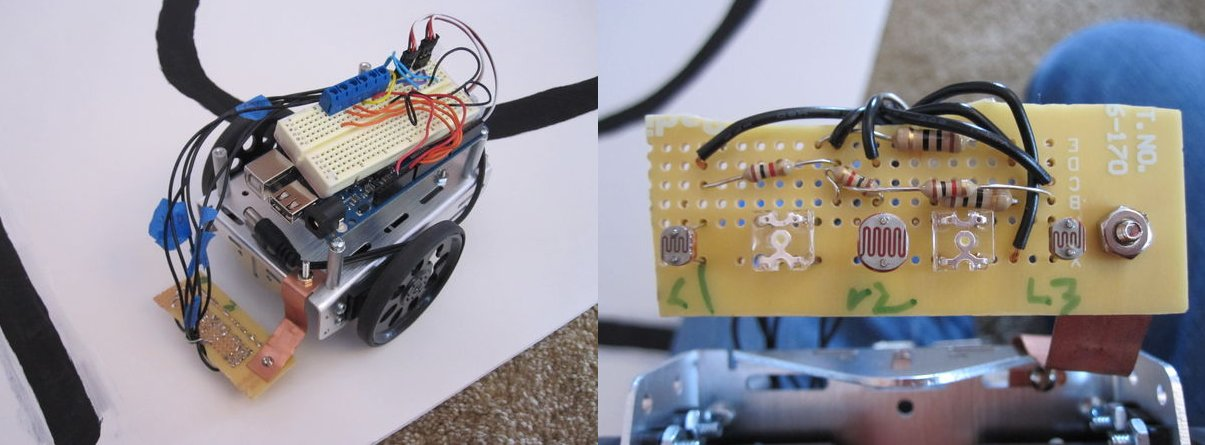
\includegraphics[width=0.7\textwidth]{boebot}
\caption[PA]{Boe Bot: Prototype (left), LDR Sensor Array (right).}
\label{fig:boebot}
\end{figure}
 
Linea is a line follower based on Arduino \cite{linea}. It is build with a robot chassis, 
infrared sensors array, two servo motors and batteries (Figure \ref{fig:linea}). Linea 
uses PID (Proportional-integral-derivative) control to compensate the misalignment from 
the line. The robot use a Pololu sensor with 8 IR leds (14 euros) which has an Arduino 
library (Right figure \ref{fig:linea}). Robot chassis uses a DF robot module (30 euros) 
which offers 2 gear motors, 2 motor sopports and 2 wheels. A motor driver from Sparkfun 
(8 euros), that can feed up to 1.2 Amperes. Others components such as ball caster, sensor 
support, batteries are also used, however, price was not added; henceforth, an estimated 
total price for Linea robot is 55 euros. 
\begin{figure}[htbp!] 
\centering    
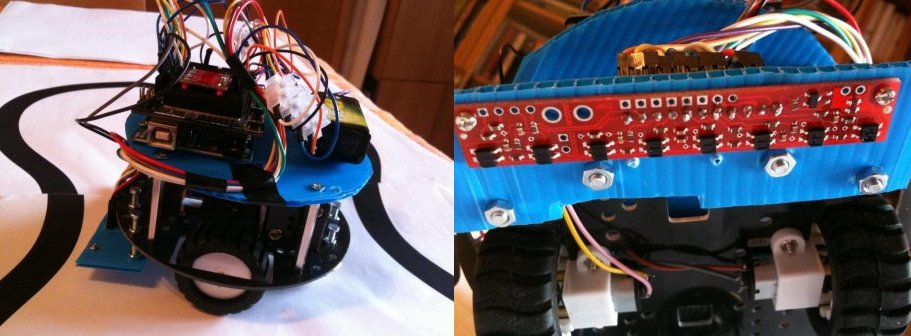
\includegraphics[width=0.6\textwidth]{linea}
\caption[PA]{Linea Robot: Prototype (left), IR Sensor Array (right).}
\label{fig:linea}
\end{figure}

Finally, ArdBot II's design is not an open-source project; nevertheless, it give access 
to the parts list and sources, Construction How-to Manual, Build Your First Robot FAQ,
Where to Get Started sources, and probably the most imporant feature the Print and Cut 
Templates in a zip file  (Rigth Figure \ref{fig:ardbotii}) and Understanding the Build 
Your First Robot Programm \cite{ardbot2}. Chassis material is fairly economical which 
cost \$ 16.95.
\begin{figure}[htbp!] 
\centering    
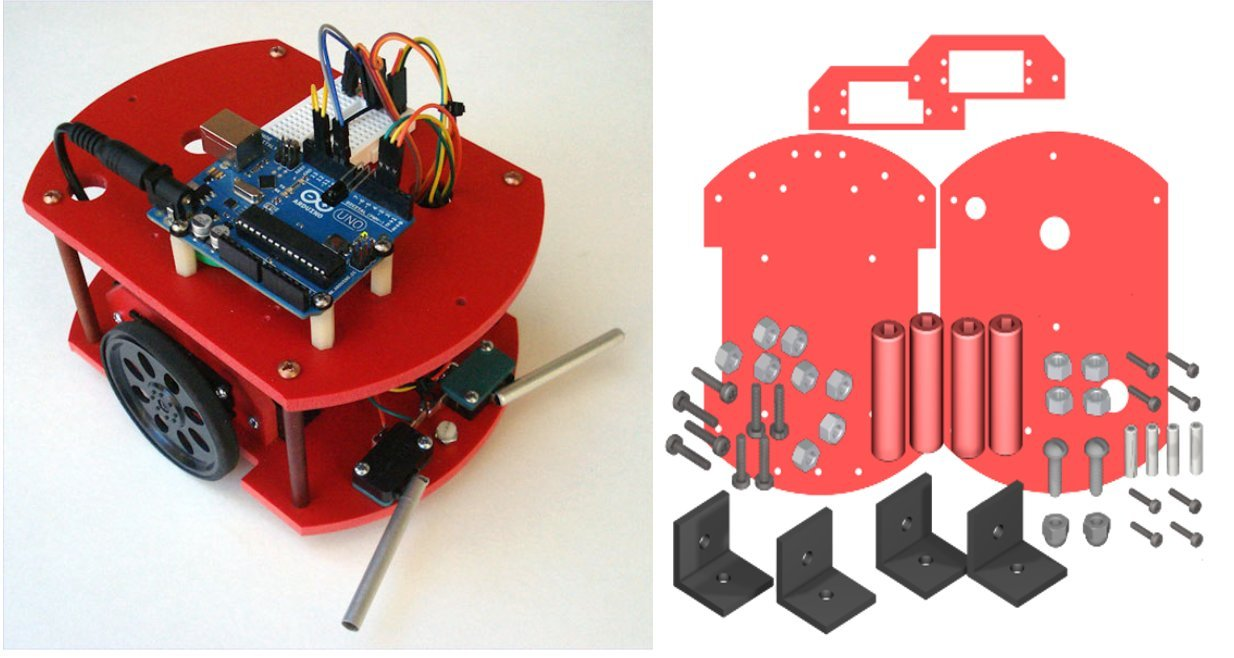
\includegraphics[width=0.6\textwidth]{ardbot2}
\caption[PA]{ArdBot II}
\label{fig:ardbotii}
\end{figure}

%----------------------------------------------------------------------
\subsection{Proposed Low-Cost Robot for {\librER}}

The first proposed low-cost robot for {\librER} is shown in Figure \ref{fig:librerobot}.
It is ensambled by using an Arduino Uno-R3 with the USB port as a power device, two Micro 
Servos TowerPro SG90 that were hacked so as to be a continuous rotation servo 
\cite{servohack1, servohack2}, two wheels (62mm of diametre), two balls caster, two LEDs, 
two LDRs, and four 100KOhms Resistors. The total cost accounts for \$  619 Mexican Pesos 
($\approx$ \$ 48 USD ). From the table \ref{t:lcr}, it can be seen detailed prices for 
the material. 
\begin{figure}[htbp!] 
\centering    
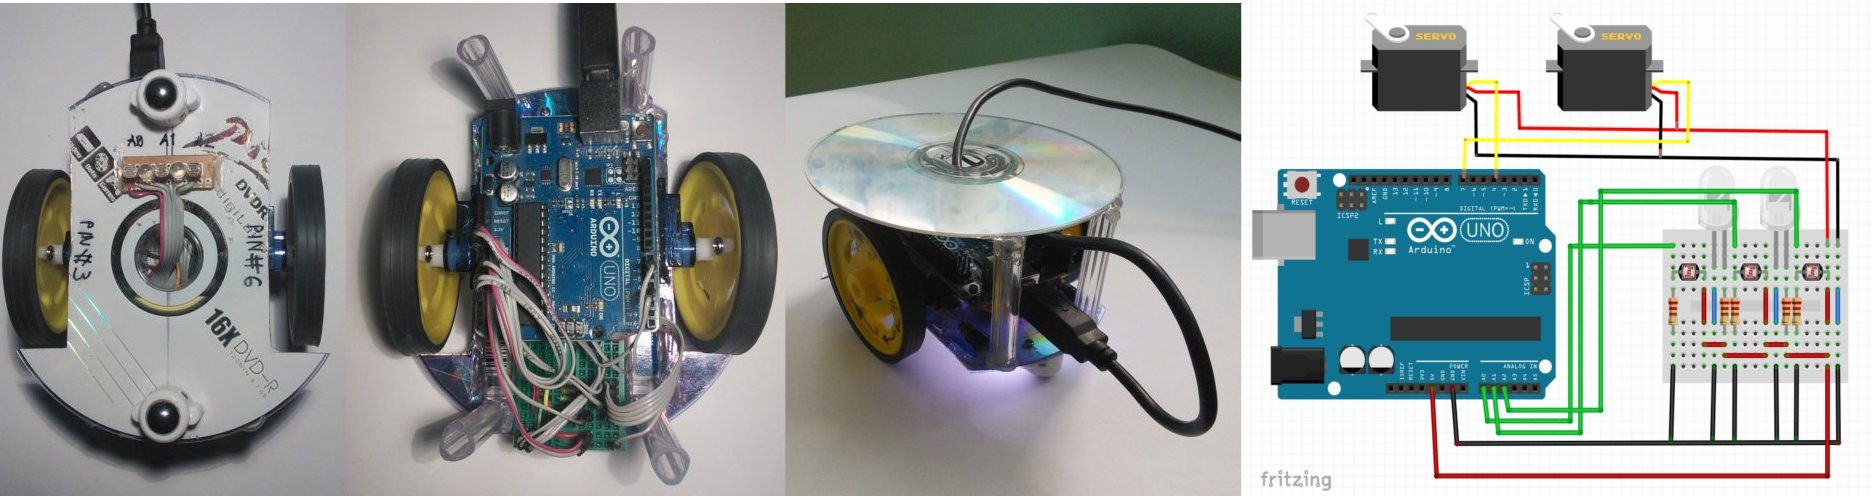
\includegraphics[width=1\textwidth]{librerobot}
\caption[PA]{Proposed Low-cost Robot: Bottom view, top view, front view and
circuit connection (From left to right).}
\label{fig:librerobot}
\end{figure}
It has been thought that total cost can be reduced since material was bought in local 
stores. Additionally, the proposed low-cost robot is under a development stage and, 
it will therefore be evolving according to the possible issues at the testing stage and 
the needs that are considered to be a very low-cost Robot.
 \begin{table}[h]
 \centering
\begin{tabular}
 { l | l }
 \toprule
 
 \textbf{Material} & Price (Mexican Pesos) \\ 
 \midrule
  
 \textbf{Arduino Uno-R3 con cable USB} & \$ 370 \\
 \textbf{2 TowerPro SG90 - Micro Servos} & \$ 160 \\
 \textbf{2 Wheels (62mm of diametre)} &  \$ 38 \\
 \textbf{2 balls caster } & \$ 82 \\
 \textbf{Breadboard - Mini Modular} &  \$ 20 \\
 \textbf{3 LDRs } & \$ 18 \\
 \textbf{2 LEDs } & \$ 10 \\
 \textbf{4 100KOhms Resistors } & \$ 1 \\
 \textbf{Total Cost} & \textbf{\$  699 ($\approx$ \$ 53.86 USD )} \\
 \bottomrule
 \end{tabular}
 \caption{Cost List of the proposed Educational Robot}
\label{t:lcr}
\end{table}
 
Furthermore, two videos were recorded so as to show demo versions of the proposed 
low-cost robot: 1) A Demo Version of the low-cost Robot using Ardublok for {\librER}  
Project, and 2)  A Voice Controlled Low-Cost Robot Using Arduino, 
PocketSphinx \cite{Pocketsphinx}, 
Firmata \cite{DrFirmata}
and Racket \cite{Racket}; 
both can be seen at \url{https://sites.google.com/site/librerobotics/videos}
 
It is worthwhile to mention that some setbacks with the non-linearity of LDR sensors 
have been faced, henceforth the line follower application has not been implemented well;
it is assumed that array sensors will work well with IR sensors. Additionally, 
the hacked servos has been presented an hysteresis behavior since the angles controls 
have a variation of 1 or 2 when sending values to stop the servos and in the case of 
speech recognition, the voice commands are sometimes misrecognized. 
 
%----------------------------------------------------------------------
\section{Software Requirements}
%----------------------------------------------------------------------

\subsection{Arduino}
The Arduino integrated development environment (IDE) is a cross-platform application 
written in Java (Figure \ref{fig:ardublockarduino}), and is derived from the IDE for 
the Processing programming language and the Wiring projects. Arduino IDE includes a code 
editor with features are: syntax highlighting, brace matching, and automatic 
indentation. It is also capable of compiling and uploading programs to the board with 
a single click. A program or code written for Arduino is called a "sketch" \cite{arduino}.

\subsection{Ardublock}
Since {\librER} is aimed to inexperienced users in coding, Ardublock is a suitable tool
which is rooted in blocks that make programming both rich interactive and less tedious. 
Ardublock is a scratch-like programming based on blocks which is reflected by its clear 
transition to text-based coding, it also generates real Arduino code in the background.
Like Arduino, Ardublock is also a run-time Java script.

Ardublock plugin can be downloaded at \cite{ardublock} and the source coude is available 
at \url{https://github.com/taweili/ardublock}. Ardublock Graphical User Interface is 
shown in Figure \ref{fig:ardublockarduino} in which three four parts are illustrated: 
programming blocks palate, zoommed out view, programming area, and arduino code. It also 
presents an example of the configuration of two servo motors that were programming in a 
loop routine of stop, counter clockwise, and clockwise. It is worth to note that settings
for the angle values may differ because of the hacked servo version.

\begin{figure}[htbp!] 
\centering    
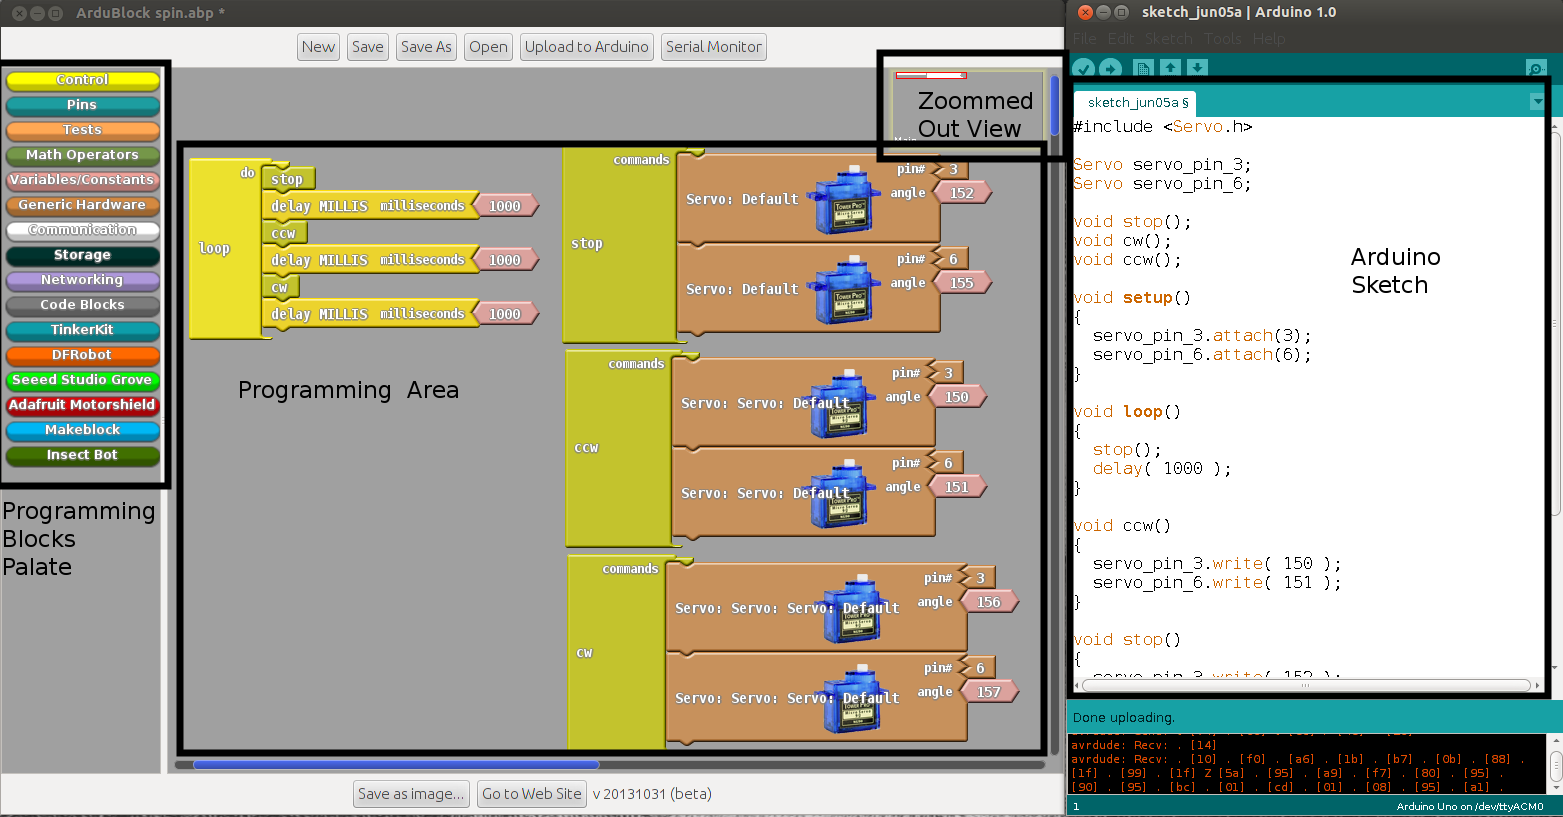
\includegraphics[width=1\textwidth]{ardublockarduino}
\caption[PA]{Examples for Ardublock and Arduino IDE}
\label{fig:ardublockarduino}
\end{figure}
 
 % Software and Hardware Requirements
%*****************************************************************************************
%*********************************** Third Chapter **************************************
%*****************************************************************************************
\chapter{Timeline}
    
 \vspace{1mm}
 \footnotesize {
 \begin{flushright}
 \textit{Lo imposible solo tarda un poco m\'as.
%Imagine a world that you would like to see in   10/100/1000  years
 }
%% \cite{auam}.
 \end{flushright}
 }
\vspace{5mm} 

Different tasks have been planned as follow:
\begin{itemize}[noitemsep,topsep=0pt,parsep=0pt,partopsep=0pt]
\item T1: Development of the Low-cost Robot
\item T2: Implement new blocks and tools to Ardublock 
\item T3: Development of the speech recognition tool with pocketsphinx, racket and firmata.
\item T4: Integration of T1, T2 and T3.
\item T5: At the first workshop of Libre Robotics adecuate surveys, methods or plans will 
	  be implemented in order to evaluate mentors and participants. In this part, it 
	  is also going to be designed the activities for the workshop with the aim of 
	  learning and sharing knowledge to build conditions for a better world.
\item T6: Week of the workshop. Evaluation of the first stage and plans for the second stage of the project.
\end{itemize}

Timeline is shown in the gantt chart (Figure \ref{fig:ganttchart}).
Document releases, low-cost robot designs, open-source software tutorials and 
web-page modifications are going to be under constant improvement and 
it is highly probably that new ideas are going to be generated during this process.

% REFERENCE FOR THE GANTT CHART COMMANDS IN LATEX
% http://www.martin-kumm.de/wiki/doku.php?id=Projects:A_LaTeX_package_for_gantt_plots

\begin{figure}[htbp!] 
\begin{center}
  \begin{gantt}{8}{16} %{rows}{columns}
    \begin{ganttitle}
      \numtitle{2014}{1}{2014}{9}
      \numtitle{2015}{1}{2015}{7}
    \end{ganttitle}
    
    \begin{ganttitle}
    \titleelement{April}{1}
    \titleelement{May}{1}
    \titleelement{Jun}{1}
    \titleelement{Jul}{1}
    \titleelement{Aug}{1}
    \titleelement{Sep}{1}
    \titleelement{Oct}{1}
    \titleelement{Nov}{1}
    \titleelement{Dec}{1}
    \titleelement{Jan}{1}
    \titleelement{Feb}{1}
    \titleelement{Mar}{1}
    \titleelement{Apr}{1}
    \titleelement{May}{1}
    \titleelement{Jun}{1}
    \titleelement{Jul}{1}
    \end{ganttitle}
    
  \ganttbar[color=green]{T1}{0}{9}
  \ganttbar[color=green]{T2}{0}{9}
  \ganttbar[color=green]{T3}{2}{7}
  \ganttbar{T4}{8}{2}
  \ganttbar{T5}{9}{6}
  \ganttbar[pattern=crosshatch,color=blue]{T6}{15}{1}
  \end{gantt}
  \caption[PA]{Gantt Chart for {\librER} project}
\label{fig:ganttchart}
  \end{center}
\end{figure}
  
 % Timeline 
%*****************************************************************************************
%*********************************** Fourth Chapter **************************************
%*****************************************************************************************

\chapter{Feeling like voluntering?}
%----------------------------------------------------------------------

\vspace{10mm}
 \footnotesize {
 \begin{flushright}
 \textit{
 We are a proudly non-profit organization driven by a culture of openness  and 
 collaboration. \\ It is a value we hold strong and it is how we work together, 
 day in and day out 
 }\cite{auam}.
 \end{flushright}
 }
\vspace{10mm}

 
People from different fields of study can help us to improve the project in different 
ways. Henceforth, some professions, possible activities and open-source software to use 
are described below.

\begin{description}[noitemsep,topsep=0pt,parsep=0pt,partopsep=0pt]
\item[Mechatronic/Electronic/Mechanical Engineers]  
to help us to design, modify, improve the proposed low-cost robot.
(Open source software/hardware to use: Arduino, BeableBone, Raspberry Pi, Blender, etc.)

\item[Computer Engineers] to help us to modify Ardublock code in order to create more 
fancy tools to inexperienced users. They are also going to help us to propose the 
computers's hardware and the process of installation. (Open source software to use: 
Ardublock, Apache Maven, Stable release of Debian, etc.)

\item[Webpage and social-network maintainers] to help us to be kindly in touch with 
subcriptors in different social networks, namely: facebook, tweeter, google+, and 
youtube. (Open source software to use: Mozilla Firefox)

\item[Graphical designers/ animator /artists] to help us to design friendly posters, 
logos, and videos. (Open source software to use: gimp, inkscape Vector, OpenShot Video 
Editor, etc.) 

\item[Architects] to help us to design a building where serendipity and comfortable 
environmental factors would be the priority. (Open source software to use: 
Sweet Home 3D)

\item[Psychologists] to help us to produce the major development of each person. For 
instance, mentors should know how to treat each participant by knowing  the answer of 
following questions: What are the potentialities of each person?. What are the necessities 
of participants who are between 10 and 15 years old?, By applying surveys to the 
participants, we can understand how to treat well each  participant in order to know 
how to communicate  better with them.

\item[Pedagogues] to help us to design free access material and develop activities 
 where organization and cooperation of the participants can foster
 possible solutions for enviromental, social awarness, the use of crop rotation,
 healthcare and animal rights issues.
 
\end{description}

In the case that your field of study or profession were not included in the previous list, 
please let us know by either sending an e-mail to \href{mailto:robotics.libre@gmail.com}
{robotics.libre@gmail.com} or contacting us at the forum 
\href{https://sites.google.com/site/librerobotics/contact-us}
{https://sites.google.com/site/librerobotics/contact-us}.













 % Feeling like voluntering
%*****************************************************************************************
%*********************************** Fourth Chapter **************************************
%*****************************************************************************************

\chapter{Future Work}
%----------------------------------------------------------------------

\vspace{1mm}
 \footnotesize {
 \begin{flushright}
 \textit{
 The present is theirs; the future, for which I really worked, is mine.
 }\\
Nikola Tesla 
 \end{flushright}
 }
\vspace{10mm}  

The following points give a brieft review of projects that
can be considered as a future work for {\librER}.
 
%----------------------------------------------------------------------
\section{Inductive Wireless Power System}
%----------------------------------------------------------------------

One of the main requirementes for educational robots is the source power that can mainly 
be covered by either onbaord batteries or an USB cable. However, batteries are 
environmental unfriendly and the USB cable is sometimes an issue for the mobility of the 
robot. Henceforth, in order to get rid of previos-mentioned drawbacks inductive wireless 
power system have proven to be the most suitable solution.
For instance, Deyle \emph{et al.} \cite{DeyleReynolds2008} in 2008 proposed a wireless 
power and bidirectional communication to a swarm of mobile robots in continuous 
operation on a bounded surface of 60cm x 60cm. Deyle's approachs is achieved by 
exciting a large, high \textit{Q} L-C resonator. Deyle compared that cost of lithium 
ion batteries and their design is very favorable. A video of their work is available at 
\url{http://vimeo.com/1900725} which shows the mini-swarm of five battery-free, 
wirelessly powered autonomous mobile robots. In the same fashion, Arunkumar 
\emph{et al.} \cite{arunkumar2010} in 2010 developed an inexpensive, low complexity 
power system capable of providing wireless power from source to sink of 
multiple mobile robots.


%----------------------------------------------------------------------
\section{Building Layout}
%----------------------------------------------------------------------

Recently, Barrett \emph{et al} \cite{Barret2013} tested 751 pupils from 34 
varied classrooms in seven different schools in the UK in which they found 
that environmental factors, namely: colour, choice, connection, complexity, 
flexibility and light, have a significant role to play in influencing academic 
performance. Henceforth, the building enviroment design is one important factor
but mainly a challenging one that few have considered so as to provide 
appropriate facilities to the learners. 
We therefore belive that the enviromental quality where activities
of {\librER} will have been taken place must consider previous-mentioned factors 
to design and build enviroments where participants can discover and develop their
own capabitilies.



% According to the results, 
% once the differences between the “worst” and “best” designed classrooms looked at in the 
% study were taken into account, it was found the be the equivalent to the progress a 
% typical pupil would be expected to make over a year.


% http://www.huffingtonpost.com/2013/01/03/school-design-student-grades_n_2404289.html

% http://www.wired.com/2013/01/school-design-grades/

% http://www.salford.ac.uk/built-environment/about-us/news-and-events/news/study-proves-classroom-design-really-does-matter

% http://www.sciencedirect.com/science/article/pii/S0360132312002582
% A holistic, multi-level analysis identifying the impact of classroom design on pupils’ learning



% http://www.ibi-nightingale.com/environment.html
% n sustainable practices, environmental design is high on our agenda. 



% 
% https://sites.google.com/site/librerobotics2015/facilities-needs
% 
% Facilities Needs
% 
% 
% (4 to 6) desktop computers (programming and website)
% (4) Work Tables at approximately 6' x 2.5' or greater.  Height ideally would be 36" high.
% (16) stools for worktables
% (8) chairs for back counter (programming, CAD and website)
% ? More Internet cables (RJ-45) + cables for any JUHSD computers for the team (one of the cables provided this weekend was cut nearly in half)
% Working Clock
% Looking for donations of these:
% (2) Heavy-Duty extension cords, approximately 25-feet
% Projector:  Looking for a permanent solution.  (We use this every meeting.  incredibly valuable for working in groups and presenting to the entire team.  4 people, for instance, can work on one program or CAD model at the same time by viewing the screen and describing thoughts, code, design to the operator.  The current projector could get reallocated at any time.  Robotics is below the priority of every curriculum need.)
% Push pins for posting robot rules, etc.
% A long list of hand and power tools (we basically have nothing at the moment)
% 




 % Future Work

% ********************************** Bibliography ******************************
\backmatter 

\begin{spacing}{0.5}
\bibliographystyle{plainnat}
\cleardoublepage
\bibliography{References/references} 
\end{spacing}

% ********************************** Appendices ********************************

\begin{appendices} % Using appendices environment for more functunality
% \include{Appendix1/appendix1}
\end{appendices}

% *************************************** Index ********************************
\printthesisindex %If index is present
\end{document}

